\setcounter{section}{0}
\section{Lý thuyết}
\subsection{Khái niệm công suất}
Công suất là đại lượng đặc trưng cho tốc độ sinh công, được tính bằng công sinh ra trong một đơn vị thời gian.
\begin{equation*}
	\calP=\dfrac{A}{t}.
\end{equation*}

Nếu vật sinh công không đều, thì công suất tính theo công thức trên gọi là công suất trung bình. 
\subsection{Đơn vị của công suất}

Trong hệ SI, công suất có đơn vị oát (watt), kí hiệu W.
\begin{equation*}
	1\ \text{W}=\dfrac{1\ \text{J}}{1\ \text{s}}.
\end{equation*}

1 watt là công suất của một thiết bị thực hiện công bằng 1 joule  trong thời gian 1 giây.

Một đơn vị khác thường được sử dụng của công suất là mã lực (CV, HP).
\begin{eqnarray*}
	1\ \text{CV}\ (\text{Pháp}) &=& 736\ \text{W}\\
	1\ \text{HP}\ (\text{Anh}) &=& 746\ \text{W}		
\end{eqnarray*}
\begin{center}
\textbf{Công suất một số hoạt động và thiết bị }
\end{center}
\begin{center}
	
	\begin{tabular}{|l|r|}
		\hline
		\multicolumn{1}{|c|}{\textbf{Tên thiết bị}} & \multicolumn{1}{c|}{\textbf{Công suất trung bình}} \\ \hline
		Tổ máy phát điện                            & $\SI{240}{MW}$                                     \\ \hline
		Tàu biển                                    & $\SI{50}{MW}$                                      \\ \hline
		Vận động viên nâng tạ $\SI{150}{kg}$        & $\SI{3.3}{kW}$                                     \\ \hline
		Máy phát thanh                              & $\SI{3}{kW}$                                       \\ \hline
		Lò nướng                                    & $\SI{2}{kW}$                                       \\ \hline
		Bóng đèn điện                               & $\SI{100}{W}$                                      \\ \hline
		Trái tim đập 60 nhịp/phút                   & $\SI{30}{W}$                                       \\ \hline
		Máy tính bỏ túi                             & $\SI{e-3}{W}$                                    \\ \hline
	\end{tabular}
	
\end{center}
\subsection{Mối liên hệ giữa công suất với lực và vận tốc}
Trường hợp vật chuyển động thẳng đều với vận tốc $v$ theo phương của lực, biểu thức liên hệ giữa công suất với lực và vận tốc là
$$\calP = \dfrac{A}{t} = \dfrac{Fs}{t}= Fv$$

\section{Mục tiêu bài học - Ví dụ minh họa}
\begin{dang}{Tính công suất trung bình trong trường hợp tổng quát}
	\viduii{2}{Một hành khách kéo đều một vali đi trong nhà ga trên sân bay trên quãng đường dài $\SI{150}{m}$ với lực kéo có độ lớn $\SI{40}{N}$ theo hướng hợp với phương ngang một góc $60^\circ$. Hãy xác định công suất của lực kéo của người này trong khoảng thời gian 5 phút.
	}
	{	\begin{center}
			\textbf{Hướng dẫn giải}
		\end{center}
		Công suất của lực kéo của người:
		$$\calP = \dfrac{A}{t} = \dfrac{Fs\cos \alpha}{t}=\dfrac{\SI{40}{\newton}\cdot\SI{150}{\meter
			}\cdot\cos\SI{60}{\degree}}{5\cdot\SI{60}{\second}}= \SI{10}{\watt}.$$
		
		\begin{center}
			\textbf{Câu hỏi tương tự}
		\end{center}
		
		Một người kéo đều một vật trên quãng đường dài $\SI{15}{m}$ theo phương ngang với lực kéo có độ lớn $\SI{20}{N}$, hướng của lực cũng theo phương nằm ngang. Hãy xác định công suất của lực kéo của người này trong khoảng thời gian 5 phút.
		
		\textbf{Đáp án:} $\SI{1}{W}$.
	}
	\viduii{2}{Một động cơ điện cung cấp công suất 15 kW cho một cần cẩu nâng 1000 kg lên cao 30 m. Lấy $g=10\ \text{m/s}^2$. Tính thời gian tối thiểu để thực hiện công việc đó.
	}
	{	\begin{center}
			\textbf{Hướng dẫn giải}
		\end{center}
		Để nâng được vật lên, cần cẩu phải tác dụng lực $F$ hướng lên trên, có độ lớn tối thiểu bằng trọng lực ($F\geq P=mg$). Lực và phương chuyển động của vật đều hướng lên nên góc giữa lực và phương chuyển động là \SI{0}{\degree}.
		
		Công mà cần cẩu đã thực hiện để nâng vật lên cao 30 m:
		\begin{equation*}
			A=Fs \cos \alpha \geq mg s\cos \alpha =\SI{1000}{\kilogram}\cdot\SI{10}{\meter/\second^2}\cdot\SI{30}{\meter}\cdot\cos\SI{0}{\degree}= \SI{300000}{\joule}=\SI{300}{\kilo\joule}.
		\end{equation*}
		Thời gian tối thiểu để thực hiện công việc đó
		\begin{equation*}
			\calP=\dfrac{A_{\min}}{t} \Rightarrow t =\dfrac{A_{\min}}{\calP}=\dfrac{\SI{300}{\kilo\joule}}{\SI{15}{\kilo\watt}}= 20\ \text{s}.
		\end{equation*}
		
		
		\begin{center}
			\textbf{Câu hỏi tương tự}
		\end{center}
		
		Một động cơ điện cung cấp công suất $\SI{0.05}{MW}$ cho một cần cẩu nâng 10 tấn lên cao 30 m. Lấy $g=10\ \text{m/s}^2$. Tính thời gian tối thiểu để thực hiện công việc đó?
		
		\textbf{Đáp án:} $\SI{60}{s}$.
		
		
	}
\end{dang}

\begin{dang}{Nêu được mối liên hệ giữa công suất với lực và vận tốc}
	\viduii{2}{Một gàu nước có khối lượng 10 kg được kéo cho chuyển động thẳng đều lên độ cao 5 m trong khoảng thời gian 1 phút 40 s. Tính công suất trung bình của lực kéo. Lấy $g=10\ \text{m/s}^2$.
	}
	{	\begin{center}
			\textbf{Hướng dẫn giải}
		\end{center}
		
		Thời gian $t=1\ \text{phút}\ 40\ \text{s} = 1\cdot\SI{60}{\second} +\SI{40}{\second}= \SI{100}{\second}$.
		
		Gàu nước chuyển động thẳng đều nên lực kéo có chiều hướng lên trên và có độ lớn đúng bằng trọng lực 
		\begin{align*}
			F=P=mg.
		\end{align*}
		Công để kéo gàu nước thẳng đều 
		\begin{equation*}
			A=Fh=mgh.
		\end{equation*}
		
		Công suất trung bình của lực kéo
		\begin{equation*}
			\calP=\dfrac{A}{t} =\dfrac{mgh}{t}=\dfrac{\SI{10}{\kilogram}\cdot\SI{10}{\meter/\second^2}\cdot\SI{5}{\meter}}{\SI{100}{\second}} =\SI{5}{\watt}.
		\end{equation*}
		
		
		\begin{center}
			\textbf{Câu hỏi tương tự}
		\end{center}
		
		Một vật có khối lượng 1,5 tấn được cần cẩu nâng đều lên độ cao $\SI{20}{m}$ trong khoảng thời gian $\SI{20}{s}$. Lấy $g=\SI{10}{m/s^2}$. Tính công suất trung bình của lực nâng của cần cẩu.
		
		\textbf{Đáp án:} $\SI{15}{\kilo\watt}$.
	}
	\viduii{2}{
		Một ô tô chuyển động thẳng đều trên đường nằm ngang với vận tốc $\SI{72}{km/h}$, công suất của động cơ là $\SI{75}{kW}$. Tính lực phát động của động cơ.
	}
	{\begin{center}
			\textbf{Hướng dẫn giải}
		\end{center}
		
		Công suất của vật chuyển động thẳng đều:
		$$\calP = Fv \Rightarrow F = \dfrac{\calP}{v} =\dfrac{\SI{75}{\kilo\watt}}{\SI{20}{\meter/\second}}= \SI{3750}{\newton}.$$
		
		\begin{center}
			\textbf{Câu hỏi tương tự}
		\end{center}
		
		Một vật khối lượng $m=\SI{10}{\kilogram}$ được kéo chuyển động thẳng nhanh dần dều trên sàn nhẵn không ma sát bằng một lực $F=\SI{5}{\newton}$ theo phương ngang từ trạng thái nghỉ. Trong thời gian 4 giây tính từ lúc bắt đầu chuyển động công suất trung bình của lực $F$ bằng
		\begin{mcq}(4)
			\item $\SI{10}{\watt}$.
			\item $\SI{8}{\watt}$.
			\item $\SI{5}{\watt}$.
			\item $\SI{4}{\watt}$.
		\end{mcq}
		
		\textbf{Đáp án: C}.
	}
\end{dang}


\section{Trắc nghiệm}
\begin{enumerate}[label=\bfseries Câu \arabic*:]
	
	\item \mkstar{1}
	
	
	{
		Công suất được xác định bằng
		\begin{mcq}
			\item giá trị công thực hiện được. 
			\item tích của công và thời gian thực hiện công.
			\item công thực hiện được trên một đơn vị chiều dài.
			\item công thực hiện được trong một đơn vị thời gian.
		\end{mcq}
	}
	
	\hideall
	{	
		\textbf{Đáp án: D.}
		
		Công suất được xác định bằng công thực hiện được trong một đơn vị thời gian.
	}
	\item \mkstar{1}
	
	
	{
		Đơn vị nào sau đây \textbf{không} phải là đơn vị của công suất?
		\begin{mcq}(4)
			\item Oát (W). 
			\item Jun/giây (J/s).
			\item Mã lực (HP).
			\item Jun (J).
		\end{mcq}
	}
	
	\hideall
	{	
		\textbf{Đáp án: D.}
		
		Jun (J) là đơn vị của công, không phải là đơn vị công suất.
	}
	\item \mkstar{2}
	
	
	{
		Một động cơ điện cung cấp công suất $\SI{15}{kW}$ cho một cần cẩu nâng vật có khối lượng 1 tấn lên cao $\SI{15}{m}$. Thời gian tối thiểu để thực hiện công việc này bằng bao nhiêu? Lấy $g=\SI{10}{m/s^2}$.
		\begin{mcq}(4)
			\item $\SI{12}{s}$. 
			\item $\SI{10}{s}$.
			\item $\SI{14}{s}$.
			\item $\SI{18}{s}$.
		\end{mcq}
	}
	
	\hideall
	{	
		\textbf{Đáp án: B.}
		
		Áp dụng công thức tính công suất:
		$$\calP = \dfrac{A}{t} \Rightarrow t = \dfrac{A}{\calP}  = \dfrac{mgs}{\calP} = \SI{10}{s}.$$
	}
	\item \mkstar{2}
	
	
	{Phát biểu nào sau đây là đúng?
		\begin{mcq}
			\item Máy có công suất lớn thì hiệu suất của máy đó nhất định cao.
			\item Hiệu suất của một máy có thể lớn hơn 1.
			\item Máy có hiệu suất cao thì công suất của máy nhất định lớn.
			\item Máy có công suất lớn thì thời gian sinh công sẽ nhanh.
		\end{mcq}
	}
	
	\hideall
	{	
		\textbf{Đáp án: D.}
		
		Công suất là đại lượng đo bằng công sinh ra trong một đơn vị thời gian. Do đó máy có công suất lớn thì thời gian sinh công sẽ nhanh.
	}
	\item \mkstar{2}
	
	
	{Một vật khối lượng $\SI{1500}{kg}$ được cần cẩu nâng đều lên độ cao $\SI{20}{m}$ trong khoảng thời gian $\SI{15}{s}$. Lấy $g = \SI{10}{m/s}^2$. Công suất trung bình của lực nâng của cần cẩu là
		\begin{mcq}(4)
			\item $\SI{15000}{W}$. 
			\item $\SI{22500}{W}$.
			\item $\SI{20000}{W}$.
			\item $\SI{1000}{W}$.
		\end{mcq}
	}
	
	\hideall
	{	\textbf{Đáp án: C.}
		
		Do nâng đều nên $F = P = mg$.
		
		Công suất trung bình của lực nâng
		
		$$\calP = \dfrac{A}{t} = \dfrac{mgh}{t} = \SI{20000}{W}.$$
	}
\end{enumerate}
\hideall
{
	\begin{center}
		\textbf{BẢNG ĐÁP ÁN}
	\end{center}
	\begin{center}
		\begin{tabular}{|m{2.8em}|m{2.8em}|m{2.8em}|m{2.8em}|m{2.8em}|m{2.8em}|m{2.8em}|m{2.8em}|m{2.8em}|m{2.8em}|}
			\hline
			1.D  & 2.D  & 3.B  & 4.D & 5.C  &   &   &   &   &   \\
			\hline
		\end{tabular}
	\end{center}
}
\section{Tự luận}
\begin{enumerate}[label=\bfseries Câu \arabic*:]
	\item \mkstar{2}
	
	
	{
		Hãy giải thích tác dụng của líp nhiều tầng trong xe đạp thể thao.
	}
	
	\hideall
	{	
		Xe đạp có líp nhiều tầng có tác dụng thay đổi chu vi của trục quay, gián tiếp thay đổi sức căng của xích, tức là thay đổi lực tác dụng, mục đích để thay đổi tốc độ của xe khi đi ở các đoạn đường khác nhau. Nhờ có líp mà ta không cần phải dùng đến bàn đạp nhiều mà bánh xe vẫn chuyển động về phía trước theo quán tính. Líp nhiều tầng ở xe đạp giúp người điều khiển xe dễ dàng đạp mà không cần mất nhiều sức. 
	}
	\item \mkstar{2}
	
	
	{
			Một hành khách kéo đều một vali đi trong nhà ga trên sân bay trên quãng đường dài $\SI{150}{m}$ với lực kéo có độ lớn $\SI{40}{N}$ theo hướng hợp với phương ngang một góc $60^\circ$. Hãy xác định công suất trung bình của lực kéo của người này trong khoảng thời gian 5 phút.
	}
	
	\hideall
	{	
		Công suất của lực kéo của người:
		$$\calP = \dfrac{A}{t} = \dfrac{Fs\cos \alpha}{t}= \SI{10}{W}.$$
	}
	\item \mkstar{2}
	
	
	{
		Một ô tô chuyển động thẳng đều trên đường nằm ngang với vận tốc $\SI{72}{km/h}$, công suất của động cơ là $\SI{75}{kW}$. Tính lực phát động của động cơ.
	}
	
	\hideall
	{	
		Công suất của vật chuyển động thẳng đều:
		$$\calP = Fv \Rightarrow F = \dfrac{\calP}{v} = \SI{3750}{N}.$$
	}
	\item \mkstar{2}
	
	
	{
		Một vật có khối lượng 1,5 tấn được cần cẩu nâng đều lên độ cao $\SI{20}{m}$ trong khoảng thời gian $\SI{20}{s}$. Lấy $g=\SI{10}{m/s^2}$. Tính công suất trung bình của lực nâng của cần cẩu.
	}
	
	\hideall
	{	
		Lực kéo của cần cẩu để nâng vật đi lên thẳng đều:
		$$F=P=mg=\SI{15000}{N}.$$
		
		Vận tốc nâng:
		$$v=\dfrac{s}{t} = \SI{1}{m/s}.$$
		
		Công suất trung bình của lực nâng của cần cẩu:
		$$\calP = Fv = \SI{15000}{W}.$$
	}
	\item \mkstar{2}
	
	
	{
		Coi công suất trung bình của trái tim là $\SI{3}{W}$. Trong một ngày - đêm trung bình trái tim thực hiện một công là bao nhiêu?
	}
	
	\hideall
	{	Đổi $\SI{24}{h} = \SI{86400}{s}.$
		
		Trong một ngày - đêm trung bình trái tim thực hiện một công là:
		
		$$A_1 = P_1t_1 = \SI{259200}{J}.$$
	}
	\item \mkstar{2}
	
	
	{
		Coi công suất trung bình của trái tim là $\SI{3}{W}$. Nếu một người sống 70 tuổi thì công của trái tim thực hiện là bao nhiêu? Một ô tô tải muốn thực hiện được công này phải thực hiện trong thời gian bao lâu? Coi công suất ô tô tải là $\xsi{3\cdot 10^5}{W}$.
	}
	
	\hideall
	{	
		
		
		Đổi 70 năm bằng 25550 ngày.
		
		Một người sống 70 tuổi thì công của trái tim thực hiện được
		
		$$A_2 = P_2t_2 = \SI{6622560000}{J}.$$
		
		Một ô tô tải muốn thực hiện công nàu phải thực hiện trong thời gian:
		
		$$t_3 = \dfrac{A_2}{P_3} = \SI{22075,2}{s} = \SI{6,132}{h}.$$
		
	}
		\item \mkstar{2}
	
	
	{
		Một người kéo một thùng nước $\SI{15}{kg}$ từ giếng sâu $\SI{8}{m}$ lên trong $\SI{10}{s}$. Hãy tính công suất của người kéo. Biết thùng nước chuyển động đều và lấy $g=\SI{10}{m/s}^2$.
	}
	
	\hideall
	{	
		Vì vật chuyển động thẳng đều nên vận tốc của vật là:
		
		$$v = \dfrac{s}{t} = \SI{0,8}{m/s}.$$
		
		Lực kéo vật lên bằng trọng lượng của vật:
		
		$$P = F = mg = \SI{150}{N}.$$
		
		Công suất của người kéo bằng:
		
		$$ \calP = Fv = \SI{120}{W}.$$
	}
	\item \mkstar{2}
	
	
	{
		Động cơ của một thang máy tác dụng lực kéo $\SI{20000}{N}$ để thang máy chuyển động thẳng lên trên trong $\SI{10}{s}$ và quãng đường đi được tương ứng là $\SI{18}{m}$. Công suất trung bình của động cơ là bao nhiêu?
	}
	
	\hideall
	{	
		Công suất trung bình của động cơ
		
		$$\calP = \dfrac{A}{t} = \dfrac{Fs}{t} = \SI{36000}{W}  = \SI{36}{kW}.$$
	}
		\item \mkstar{3}
	
	
	{
		Một ô tô khối lượng 1 tấn đang hoạt động với công suất $\SI{5}{kW}$ và chuyển động thẳng đều với vận tốc $\SI{54}{km/h}$ thì lên dốc. Hỏi động cơ ô tô phải hoạt động với công suất bằng bao nhiêu để có thể lên dốc với tốc độ như cũ? Biết hệ số ma sát giữa bánh xe và mặt đường không đổi, dốc nghiêng góc $\SI{2,3}{^\circ}$ so với mặt đường nằm ngang và $g = \SI{10}{m/s}^2.$
	}
	
	\hideall
	{	
		Đổi 1 tấn $= \SI{1000}{kg}; \SI{5}{kW} = \SI{5000}{W}; \SI{54}{km/h} = \SI{15}{m/s}.$
		
		Khi xe ô tô chuyển động thẳng đều: 
		
		$$F'_\text{ms} = F'_\text{k} = \dfrac{\calP'}{v} = \xsi{{1000}{3}}{N}.$$
		
		Hệ số ma sát là:
		
		$$\mu = \dfrac{F'_\text{ms}}{mg} = \dfrac{1}{30}.$$
		
		Khi ô tô chuyển động lên dốc, các lực tác dụng lên ô tô được biểu diễn 
		
		
		\begin{center}
			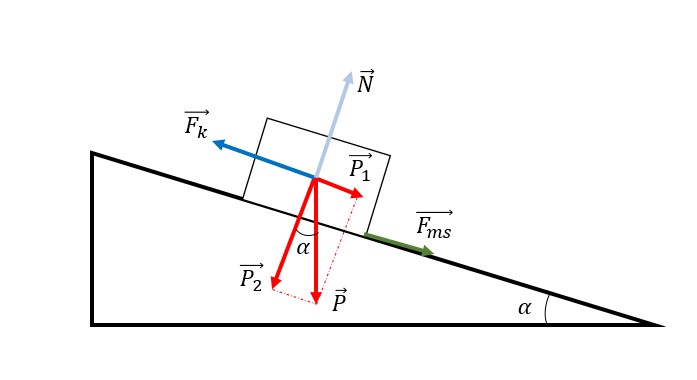
\includegraphics[scale=0.8]{../figs/VN10-2022-PH-TP027-1.jpg}
		\end{center}
	
		Khi lực kéo ô tô khi lên dốc có giá trị
		$$F_\text{k} = F_\text{ms} + P_1 = \mu mg \cos \alpha + mg\sin \alpha = \SI{734,38}{N}.$$
		
		Để có thể lên dốc với tốc độ như cũ, ô tô phải hoạt động với công suất
		
		$$\calP = F_\text{k} v = \SI{11015,7}{W}.$$
	}
	\item \mkstar{2}
	
	
	{
		Một gàu nước có khối lượng $\SI{15}{kg}$ được kéo cho chuyển động thẳng đều lên độ cao $\SI{5}{m}$ trong khoảng thời gian 1 phút 15 giây. Tính công suất trung bình của lực kéo. Lấy $g = \SI{10}{m/s}^2$.
	}
	
	\hideall
	{	
		Vận tốc của gàu nước:
		
		$$v = \dfrac{s}{t} = \xsi{\dfrac{1}{15}}{m/s}.$$
		
		Công suất của lực kéo bằng
		
		$$\calP = Fv = mgv= \SI{10}{W}.$$
	}

\end{enumerate}